%; whizzy chapter
% -initex iniptex -latex platex -format platex -bibtex jbibtex -fmt fmt
% 以上 whizzytex を使用する場合の設定。


%     Tokyo Debian Meeting resources
%     Copyright (C) 2006 Junichi Uekawa

%     This program is free software; you can redistribute it and/or modify
%     it under the terms of the GNU General Public License as published by
%     the Free Software Foundation; either version 2 of the License, or
%     (at your option) any later version.

%     This program is distributed in the hope that it will be useful,
%     but WITHOUT ANY WARRANTY; without even the implied warranty of
%     MERCHANTABILITY or FITNESS FOR A PARTICULAR PURPOSE.  See the
%     GNU General Public License for more details.

%     You should have received a copy of the GNU General Public License
%     along with this program; if not, write to the Free Software
%     Foundation, Inc., 51 Franklin St, Fifth Floor, Boston, MA  02110-1301 USA

%  preview (shell-command (concat "xpdf " (replace-regexp-in-string "tex$" "pdf"(buffer-file-name)) "&"))
% 画像ファイルを処理するためにはebbを利用してboundingboxを作成。
%(shell-command "cd image200611; ebb *.png")

%%ここからヘッダ開始。

\documentclass[mingoth,a4paper]{jsarticle}
\usepackage[dvipdfmx]{graphicx}
\usepackage{fancybox}
\usepackage{longtable}
\usepackage{ascmac}	% 囲み (screen,itembox)
\usepackage{fancyvrb}   % 囲み Verbatim のために必要
\usepackage[dvipdfmx]{hyperref}
\usepackage{url}
\usepackage[dvipdfmx]{color}

%http://www.naney.org/diki/dk/hyperref.html
%日本語EUC系環境の時
\AtBeginDvi{\special{pdf:tounicode EUC-UCS2}}
%シフトJIS系環境の時
%\AtBeginDvi{\special{pdf:tounicode 90ms-RKSJ-UCS2}}

%% spacing の設定をする。外枠を減らす。
\setlength\headheight{0mm}
\setlength\topmargin{-20mm}
\setlength\headsep{0mm}
\setlength\topskip{3mm}
\setlength\maxdepth{4pt}
\setlength\columnsep{6mm}
\setlength\textheight{252mm}
\setlength\topmargin{-5mm}
\setlength\textwidth{170mm}
\setlength\oddsidemargin{-5mm}
\setlength\evensidemargin{-5mm}

% commandline環境を定義。画面入出力についてはcommandline環境
% で表記する
\newenvironment{commandline}%
{\VerbatimEnvironment
  \begin{Sbox}\begin{minipage}{15cm}\begin{fontsize}{7.3}{7.3} \begin{BVerbatim}}%
{\end{BVerbatim}\end{fontsize}\end{minipage}\end{Sbox}
  \setlength{\fboxsep}{8pt}\fbox{\TheSbox}}


%%% start of santaku
\makeatletter
\newwrite\tf@jqz
\immediate\openout\tf@jqz\jobname.jqz\relax
\makeatother
\newcounter{santakucounter}
\newcommand{\santaku}[5]{%
\addtocounter{santakucounter}{1}

\addtocontents{jqz}{\arabic{santakucounter}. #5\\}
\begin{minipage}{1\hsize}
問題\arabic{santakucounter}. 
#1\\
□ A #2\\
□ B #3\\
□ C #4
\end{minipage}
\hspace{1cm}
\\

}
%%% end of santaku

\newcommand{\emptyspace}{(\underline{\hspace{1cm}})}

\newcommand{\subsubsubsection}[1]{%
\vspace{1zw}{\bf #1}\\}


% sectionをセンタリングする
\makeatletter
  \renewcommand{\section}{\@startsection{section}{1}{\z@}%
    {\Cvs \@plus.5\Cdp \@minus.2\Cdp}% 前アキ
    {.5\Cvs \@plus.3\Cdp}% 後アキ
    {\normalfont\Huge\headfont\raggedright\centering}} % style
\makeatother

% section の代わりの環境
\newcommand{\dancersection}[2]{%
\newpage
東京エリアDebian勉強会 2006
\hrule
\vspace{0.5mm}
\hrule
%\hfill{}
\includegraphics[width=3cm]{image200502/openlogo-nd.eps}\\
\hfill{}
\includegraphics[width=16cm]{image2006-natsu/guruguru-sand-light.png}\\
\vspace{-5cm}
\begin{center}
\section{#1}
\end{center}
\hfill{}\colorbox{white}{#2}\hspace{3cm}\space\\
\vspace{1cm}
\hrule
\vspace{0.5mm}
\hrule
\vspace{1cm}
}

% for dancerj
\newcommand{\fgref}[1]{図\ref{#1}}
\newcommand{\tbref}[1]{表\ref{#1}}


\begin{document}

\begin{titlepage}

% 毎月変更する部分, 本文の末尾も修正することをわすれずに
\title{
 第22回 東京エリア Debian 勉強会\\事前資料}
\date{2006年11月19日}
\author{Debian勉強会会場係 上川 純一\thanks{Debian Project Official Developer}} 
\maketitle
\thispagestyle{empty}
\end{titlepage}

\newpage
\tableofcontents

\dancersection{Introduction To Debian 勉強会}{上川 純一}

今月のDebian勉強会へようこそ。
これからDebianのあやしい世界に入るという方も、すでにどっぷりとつかってい
るという方も、月に一回Debianについて語りませんか?

目的として下記の二つを考えています。

\begin{itemize}
 \item メールではよみとれない、もしくはよみとってられないような情報を情
       報共有する場をつくる
 \item まとまっていないDebianを利用する際の情報をまとめて、ある程度の塊と
       して出してみる
\end{itemize}

また、東京にはLinuxの勉強会はたくさんありますので、Debianに限定した勉強
会にします。Linuxの基本的な利用方法などが知りたい方は、他でがんばってくださ
い。
Debianの勉強会ということで究極的には参加者全員がDebian Packageを
がりがりと作りながらスーパーハッカーになれるような姿を妄想しています。

Debianをこれからどうするという能動的な展開への土台としての空間を提供し、
情報の共有をしたい、というのが目的です。
次回は違うこと言ってるかもしれませんが、御容赦を。

\subsection{講師紹介}

\begin{itemize}
 \item{上川 純一} 宴会の幹事です。
\end{itemize}

\subsection{事前課題紹介}

今回の事前課題は
「Debian勉強会で知りたいこと、今日の質問」
というタイトルで200-800文字程度の文章を書いてください。
というものでした。
その課題に対して下記の内容を提出いただきました。

\subsubsection{山下さん}

Debian勉強会で知りたいことは、メーリングリストやIRCでは普段聞けない、裏
事情など。8月に東京で参加したときに、みなさんがときどき、ぼそっと言われ
る発言が非常に参考になったので。

気になっていた事なんですが、Windows上のEclipseに比べて、Debian上の方が若
干重たく感じます。Java関係の問題だと思うのですが。今後、関西でのDebian勉
強会の頻度について。

\subsubsection{谷口さん}

普段、windowsをメインに使っていまして、サブとしてredhat、fedora、vine な
どのredhat系のosあるいはfreebsdを使っている、あるいは使ったことがあるの
ですが、debianを使ったことは無く、debianの知識はほとんどありません。本勉
強会でdebianの特徴やその良さについて知ることが出来ればと思っています。特
にパッケージ関連の話について詳しく知りたいです。質問に関しては、その場で
気になった点を質問させていただくと思います。

\subsubsection{岩本さん}

 debianではetchから文字コードがUTF-8が標準になると聞いております、UTF-8
化によるメリット、デメリットやインストゥール時やアプリケーション動作時に
気をつけるべきところなどがありましたら教えていただきたく思います。

 また、最近のノートパソコンにdebian eachをインストゥールするとすれば、
この勉強会に参加されている方はどんな機種を選択するのかお聞きしたい。(ノー
トパソコン購入時の参考にしたい為。)

\subsubsection{榎 真治さん}

普段あまりDebianを使いこなせていないのですが、特有の流儀というものがある
と感じております。

勉強会に参加することでそれを知る手がかりになればと思っております。

\subsubsection{Yutaka Kametaniさん}

たくさんのディストリビューションがある中で、デビアンを使うメリットは何で
すか?

\subsubsection{畑中さん}

研究室配属時に、Debianを使ってもらうと先生からいわれ、とりあえず自分のコ
ンピュータにインストールをしてみました。これが初めての純正Debianです。他
のディストリビューションにあるようなGUIインストールや、GUIでのaptなど(実
はあったらごめんなさい)がなく、Linux初心者にインストールさせるには、多少
敷居が高いと思えました。そのあたりの開発はされているのでしょうか。

\subsubsection{Takashi Hamabeさん}
私はdebianを使い始めて間もなく、自分自身まだまだ勉強が足りないと思っています。
そのことで大変な失礼があるかと思いますが、恥ずかしながら質問したいと思います。
どうしてdebianを開発しようと思ったのでしょうか?
どうして使う側ではなく、開発側にまわろう思ったのでしょうか?
開発側にまわるためには、やはり大変な努力と知識が必要だと思いますが、何がそういう努力をさせるような情熱を与えてくれるのでしょうか?

\subsubsection{藤澤 恵一朗さん}

Debianを使ってみて最初に思ったのはXが軽いなあという点です。学科指定のFedora3やFreeBSDではもっさり感があったのですが、Debianは快適です。普通にコンパイルしただけでなくて、何かチューニングしているのでしょうか。

aptでいれたpackageが確実に削除できるのがすごいなあと思いました。心おきなくいろんなものを試せるので勉強もしやすいです。

違和感があったのは、apacheやproftpdなどはaptでいれると必ず自動起動するという点です。FreeBSDでは設定をしないと起動しなかったので、apacheのバージョン違いをいれたりしても動作的には問題がなかったです。しかしDebianはどういった挙動をとるのかわからないので不安です。Debianの勉強不足というのが一番の理由ですが、なぜこうしているのか気になります。

\subsubsection{乾さん}

Debianは最近使い始めたのでまだよくわかっていません。
今回の勉強会では、debianの魅力について教えてもらえたらと思います。できれば他と比べての欠点も知りたいです。

\subsubsection{久松さん}

2点あります。
\begin{enumerate}
 \item  ネットワークの設定方法\\
 ネットワークが変わるたびに、 /etc/init.d/netwoking stop;
 /etc/network/interfaces の書き換え、/etc/init.d/netwoking start と、
 shell script を使ってやっています。我ながらこれは美しくないと思っており、
 美しいやり方を教えて頂きたいです。
 \item  apt、aptitude の使い方\\
 私は、パッケージをインストール、または削除するときに、apt、aptitude で
 目的のパッケージを選択しづらく、dselect のみを使っています。apt は、パッ
 ケージ名を正しく書く必要があり、使いづらいです(パッケージ名を書き間違
 えることが、かなりある)。aptitude は、パッケージがどの分類に属すか、分
 からないときがある(意外と間違える)。また、文字列の検索でパッケージを
 選択できるが、文字列がヒットしたパッケージ名が、"Search for:" というウィ
 ンドウの陰に隠れていて、使いにくい(もっと文字列を追加するべきなのか?こ
 れで十分なのか、判断できない)。dselect は、インクリメンタルサーチが使え
 たら、特になにもいうことはないです。おそらく、私の使い方が間違っている
 と思うので、apt、aptitudeの使い方をご教授いただけたら幸いです。
\end{enumerate}

\subsubsection{岩松 信洋}

\begin{itemize}
 \item  Debian 開発者の開発環境(家のPCは15台あって、xDSL回線は3本ありますとか。)
	紹介とか、いつごろ寝ているのか、机の上はどんな汚さなのか、公開できる範囲の私
	生活を知りたいです。
	
 \item 関西でのDebian 具合\\
	関西出身の自分としては関西でのDebianの浸透っぷりを知りたいです。
\end{itemize}

\subsubsection{上川}

今日の私の興味は、Debian 勉強会を関西で開催できるのか、どういう人がいる
のか、ということを確認することです。Debianについて活発に関西でもイベント
など開催されるとよいなぁ、と希望しています。

%%% trivia quiz
\dancersection{Debian Weekly News trivia quiz}{上川 純一}

ところで、Debian Weekly News (DWN)は読んでいますか?
Debian 界隈でおきていることについて書いているDebian Weekly News.
毎回読んでいるといろいろと分かって来ますが、一人で読んでいても、解説が少
ないので、
意味がわからないところもあるかも知れません。みんなでDWNを読んでみましょう。

漫然と読むだけではおもしろくないので、DWNの記事から出題した以下の質問にこたえてみてください。
後で内容は解説します。

\subsection{2006年40号}
\url{http://www.debian.org/News/weekly/2006/40/}
にある10月31日版です。

\santaku
{Frank K\"usterがカーネル 2.6.18 パッケージについて発表したのは?}
{まだ安定していないけどどんどん利用してください}
{General Resolution の結果、 Linuxじゃないカーネルを今後利用する}
{firmware blob を Debian package に含めるようにした}
{C}

\santaku
{mplayer パッケージになにがおきたか?}
{NEW キュー滞在時間の新記録をさらに更新した}
{Debian unstable に入った}
{もうあきらめることになった}
{B}

\dancersection{最近のDebian関連のミーティング報告}{上川 純一}

\subsection{東京エリアDebian勉強会21回目報告}
% (query-replace-regexp "<.*>" "")

   	  東京エリアDebian勉強会報告。
	  10月の第21回Debian勉強会を実施しました。
	    Extramadura の報告、flash の紹介、および apt のプロファイリングの結果について報告しました。
	  
	  今回の参加人数は23人くらいでした。
	  
	  参加者は小林さん、柏木さん、倉澤さん、前田さん、須藤さん、武藤さん、やまねさん、野首さん、小室さん、高杉さん、えとーさん、
	  吉田@板橋さん、八田さん、キタハラさん、ごとうまさのりさん、中野さん、ysjj さん、松山さん、河内さん、David Smith さん、
	  Charles Plessy さん、上川でした。
        
	
	  
	    まず、事前課題の紹介をしました。
	    ネットワークの設定については、皆思うところがあるようです。
	    GUIのツールなどが実は整備されていて、それをみんなしらないだけなのではないか?という話が出ました。
	    また、NTLM認証のプロキシに対応していないアプリケーションが多数あるんじゃないか、HTTPSが重要なんじゃないのか、
	    という話題が出ました。
	    Debconf の会場がNTLM Proxy 必須で、さらにスケジュールが HTTPS RSS で流れるようになっていたら、
	    Debian のそこらへんのサポートも改善するんじゃないか、という提案が出てみたり。
	  
	  
	    恒例のクイズ、今回5問しかありませんでした。
	    Debian Weekly News が休止してしまったのです。今後クイズのネタがなくなって非常に困りますが、どうしましょう?
	  
	  
	    武藤さんが Extramadura i18n 会議について発表しました。
	    pootle はまだ即使えるという状況ではないということは残念で
	    すが、今後タスクフォースとしてまとまっていろいろとやってい
	    こうという気概と雰囲気がかんじられるので期待です。
	  
	  
	    松山さんに flash ming ネタを発表してもらいました。
	    ming を使うことはできるのですが、結構苦戦した、という話でもりあがりました。
	    野首さんが、 ming ネタについてあつく語っていました。
	    一子相伝の技の次世代への継承が行われているところに出くわした感じです。
	  
	  
	    上川が apt のプロファイリングのネタについて発表しました。
	    SHA1のチューニングについては、意外とできないものだ、という結論で終わりました。
	  
	  
	    今回宴会は「えん屋」で行いました。
	    店はけむたかったけど、みなさんといろいろと話ができて、おもしろかったです。
	  

\dancersection{パッケージングについて}{岩松 信洋}
\label{sec:iwamatsupackaging}
\subsection{パッケージングについての基礎知識}

パッケージングとは、無数に存在するソフトウェアの配布したりソ
フトウェアのバージョンを管理するために、ファイルなどをまとめ
たものです。
それらをサポートするシステムがあり、パッケージ管理システムといいます。

例えば、あるフリーソフトウェアを入手し、使おうとした場合、 

\begin{commandline}
% ./autogen.sh
% ./configure
% make 
# make install
\end{commandline}  


として、ライブラリ等をチェック、コンパイル、インストールという作業を行う必要が
あります。
これらの過程でライブラリのチェックで新たにライブラリが必要だったり、コンパイル
できなかったりする事が多々あります。
もし、パッケージングシステムを使って、ソフトウェアを構成していた場合は、これら
の問題を解決したり、ソフトウェアを容易に使用することができるようになります。

パッケージングシステムの必要な機能として
\begin{itemize}
	\item パッケージに関する情報
	\item パッケージの作成
	\item パッケージのインストール
	\item パッケージの更新
	\item パッケージのアンインストール
\end{itemize}
があります。

ソフトウェアをパッケージングし、インストールやアンインストール、ソフトウェアの
アップデートなどを容易に行う事が目的です。

ここで重要なのが、ユーザーだけが容易に使用できるということではなく、開発者側と
しても容易にパッケージングを行い、パッケージをメンテナンスできるということです。

%今回は開発者側からみたパッケージングについて書いていこうと思います。

%このパッケージングされたものを使用することにより楽をしようということなのです。


\subsection{Debian でのパッケージ管理/Debian パッケージについて}

\subsubsection{dpkg}

	Debian では dpkg と呼ばれる Debian パッケージ管理システムを使用しています。
	この dpkg を Debian の基礎としているため、Debian で配布されている全てのパッ
	ケージは .deb ファイル形式で提供されてなければなりません。
	
	dpkg では
	\begin{enumerate}
		\item 依存関係の解決

			\begin{itemize}
				\item Depends                 依存
				\item Recommends              推奨
				\item Suggests                提案
				\item Conflicts               競合
				\item Provides                提供
				\item Replaces                置換
			\end{itemize}

		\item パッケージバージョンによるアップグレードのサポート

		\item インストール前後、アンインストール前後の設定機能
	\end{enumerate}
	などが提供されています。

\subsubsection{Debian Policy}

	Debian で配布されるパッケージは、厳格なパッケージポリシー Debian Policy 
	\footnote{http://www.debian.org/doc/debian-policy} に基づいて作成されている必要があります。\\
	この Debian Policy によって、パッケージの互換性が保たれています。

\subsubsection{パッケージの種類}
	Debian で配布されるパッケージは、DFSG ( Debian Free Sofware Guideline )によって3つのセクションに分けられます。
	DFSG は Debian として Free Software とはどのようなものなのか、定義するものです。

	\begin{enumerate}
		\item main

			DFSG に適合したパッケージは main セクションに置かれます。
		\item contrib

			DFSG に適合しているが、non-freeなパッケージに依存しているパッケージは contrib セクション
			に置かれます。
		\item non-free

			DFSG に適合しないパッケージは non-free セクションに置かれます。
			non-freeのパッケージは Debian の一部ではありません。
	\end{enumerate}

	 さらにこれらのパッケージを用途に応じて分けられています。

	
\subsubsection{apt}

	最近は dpkg を直接使い、パッケージをインストールすることは少なくなっています。
	変わりにAPT\footnote{Advanced Package Tool)}を使うようになりました。 
	その理由として、提供されるパッケージが増え、依存関係が複雑になって必要なパッケージをダウンロードするのが
	大変になってきためです。そこで開発されたのが、パッケージをまとめて管理する apt です。
	dpkg 用のフロントエンドになっており、中では dpkg が呼ばれています。
	
	APTの役目として
	\begin{itemize}
		\item パッケージの管理

			パッケージをどのようにインストール、アンインストールをするか考える。
		\item パッケージをダウンロードする。
		\item パッケージの検索を行う。
	\end{itemize}

	があります。Debian Policy に基づいて 作成されているからこそ実現できています。。

\subsection{Debian でパッケージを作る際のツール群}

	Debian でパッケージングを行うためのサポートするソフトウェアがあります。
	パッケージングを行い、品質の高いパッケージを作るために以下のソフトウェア
	が提供されています。

\subsubsection{dpkg-dev}
	このパッケージには Debian ソースパッケージを展開、構築、アップロードするために必要なツール群をまとめたものです。
	ソースパッケージの展開に必要な dpkg-source や パッケージの作成に必要なdpkg-buildpackage が入っています。
  
\subsubsection{debhelper}

	dh\_xxx というパッケージ作成をサポートツールをまとめたものです。
	Debian 魔窟のひとつです。

\subsubsection{devscript}

	debuild などのパッケージ作成フロントエンドが提供されています。
	
\subsubsection{dh-make}
	ソースパッケージの雛型を作るツールです。
	ソースパッケージやバイナリパッケージを作成するために最低限必要なファイルを生成してくれます。
	perl や php 用の雛型を作成する dh-make も存在します。

	
\subsubsection{lintian}	
	Debian パッケージ用のチェッカーです。
	Debian Policy にあわせて作られています。
	linda というパッケージ用チェッカーもあります。lintian は Perl で、linda は Python でプログラミング
	されたものです。

\subsubsection{fakeroot}
	fakeroot は root 権限をシミュレートします。パッケージは、root の所有権
	でファイルがインストールされている必要があります。fakeroot を使用することによって、
	root にならずにパッケージを構築できます。  

\subsubsection{cdbs}
	Common Debian Build System。
	dh\_xxx などをまとめて、簡潔にパッケージ作成スクリプトを記述することができるようにするためのソフトウェア。
	
\subsubsection{GnuPG}
	作成されたパッケージにサインするために使います。
	そのパッケージがたしかにそのメンテナの PGP key によって作られていることを証明するためです。
	
\subsubsection{dpatch}

	Debianのソースパッチを管理するツールです。
	Debian パッケージの差分は *.diff.gz という差分ファイルとして管理されるため、 どの部分がどういうパッチであるか
	ということを管理していません。 その部分を実装するのが dpatch です。

%\subsubsection{pbuilder}
%	パッケージの作成をチェックするためのソフトウェアです。
%	最低限のユーザーランドで構成され、依存関係にかかれた必要なパッケージをダウンロードし
%	パッケージをビルドします。	

\subsection{実際にパッケージを作成してみる}

	Debian 用のパッケージを作成する方法を簡単に説明します。	
	今回のパッケージ化の説明で使用するソフトウェアは cairo-dock\footnote{http://www.gnome-dock.org/trac} 
	というMac OS X Dock風のDockアプリケーションです。
	
	\begin{center}
		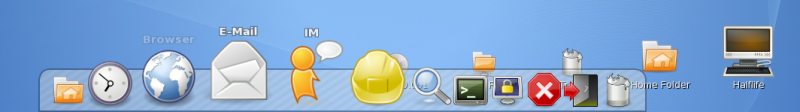
\includegraphics[width=0.5\hsize]{image200611/cairo-dock-ss.png}
	\end{center}

	Debian では\footnote{パッケージを管理しているディストリビューションでも使われています。}
	開発元、オリジナル配布元のことを Upstream といいます。

\begin{enumerate}

	\item パッケージ化を行うためにパッケージをインストールします。

	\begin{commandline}
# apt-get install dh-make devscripts debhelper dpkg-dev dpatch 
	\end{commandline}

	\item ソフトウェアのソースコードをダウンロードし、展開します。
		
	\begin{commandline}
% wget http://www.gnome-dock.org/prerelease/cairo-dock-0.0.1b.tar.gz
% tar -xzf cairo-dock-0.0.01b.tar.gz
	\end{commandline}

	\item 展開した後、ディレクトリ名を パッケージ名-パッケージのバージョン になるようにに修正します。

	\begin{commandline}
% ls -l 
drwxr-xr-x  2 iwamatsu iwamatsu    1024 2006-08-09 01:29 cairo-dock
-rw-r--r--  1 iwamatsu iwamatsu  107560 2006-08-09 01:30 cairo-dock-0.0.1b.tar.gz

% mv cairo-dock cairo-dock-0.0.1b
	\end{commandline}

		すでに行われている場合は行う必要はありません。

	\item バックアップファイルや実行ファイルが残っているので、消しておきます。

	\begin{commandline}
% ls
Makefile       clock.svg        folder.svg         lowfat.svg           start-cairo-dock.sh~  terminal.svg
cairo-dock     configure.scan   gnome-fs-home.svg  movies.svg           sticky-notes.svg      user-home.svg
cairo-dock.c   development.svg  im.svg             music.svg            stop.svg              user-trash-full.svg
cairo-dock.c~  editor.svg       lockscreen.svg     search.svg           tango-colors.h        web-browser.svg
chat.svg       email.svg        logout.svg         start-cairo-dock.sh  tango-colors.h~
% make clean
	\end{commandline}
	\item 対象のソフトウェアのディレクトリに移動し、dh\_make --createorigを実行します。

		dh\_make を実行したときに、パッケージの種類を選択します。
		\begin{itemize}
			\item single binary

				ひとつのバイナリパッケージを作成する。
			\item multiple binary
				
				複数のバイナリパッケージを作成する。
			\item library

				ライブラリ用のパッケージを作成する。
			\item kernel module
		
				カーネルモジュール用のパッケージを作成する。
			\item cdbs
		
				cdbs ( Common Debian Build System ) を使ったパッケージを作成する。
		\end{itemize}
		

		実行すると、debian ディレクトリが作成されます。
		--createorig を指定しない場合はオリジナル用のディレクトリ( 今回の場合は cairo-dock-0.0.1b.orig )が作成されません。
		このディレクトリがない場合は、ソースパッケージの一部として配布される .orig.tar.gz が生成されません。

	\begin{commandline}
% dh_make --createorig

Type of package: single binary, multiple binary, library, kernel module or cdbs?
 [s/m/l/k/b] s

Maintainer name : Nobuhiro Iwamatsu
Email-Address   : hemamu@t-base.ne.jp
Date            : Fri, 17 Nov 2006 07:30:18 +0900
Package Name    : cairo-dock
Version         : 0.0.1b
License         : blank
Type of Package : Single
Hit <enter> to confirm:
Done. Please edit the files in the debian/ subdirectory now. You should also
check that the cairo-dock Makefiles install into $DESTDIR and not in / .
	\end{commandline}
	
	\item debianディレクトリ内を編集します。

		dh\_make を行ったあとの debian ディレクトリは以下のようになっています。
		これらはテンプレートファイルなので、パッケージによって必要のないものも含まれています。
		\begin{itemize}
			\item README.Debian

				Debian 固有のREADME			           
			\item changelog
  
				Debian 固有の変更履歴
			\item copyright
 
				ソフトウェアのライセンスとコピーライト 
			\item docs    
            
				/usr/share/doc にインストールされるファイルのリスト
			\item emacsen-startup.ex
			\item emacsen-install.ex
			\item emacsen-remove.ex
       
 				xemacs 用テンプレート
			\item postinst.ex
			\item postrm.ex
			\item preinst.ex         
			\item prerm.ex

				インストール、アンインストール時に実行されるスクリプトテンプレート
			\item cairo-dock-default.ex
  
				/etc/init.d/用のテンプレート

			\item compat     
			\item cron.d.ex
  
				crond 用のテンプレート
			\item init.d.ex
           
				/etc/init.d/用のテンプレート
			\item rules

				パッケージ作成用 Makefile
			\item cairo-dock.doc-base.EX  

				docbook 用のテンプレート
			\item control
    
				パッケージのメタ情報
			\item dirs
			\item manpage.xml.ex 
			\item manpage.sgml.ex       
			\item manpage.1.ex
        
				manpages のテンプレート
			\item menu.ex
          
				menu システム用テンプレート
			\item watch.ex

				upstream 監視用設定テンプレート
		\end{itemize}
		
		
	\item *.ex および *.EX ファイルを削除します。

		今回のソフトウェアのパッケージ化には *.ex や *.EX は必要ないので、削除します。
 
	\item control ファイルの編集

		control ファイルを編集します。
	\begin{itemize}
		\item Source	

			ソースパッケージ名を記述します。
			今回は ソースの名前から cairo-dock とします。

			詳細は Debian-Policy の {\bf 5.6.1 Source} を参照してください。
		\item Section

			パッケージの種類を指定します。
			cairo-dock は x11 用のソフトウェアなので、x11 とします。

			詳細は Debian-Policy の {\bf 2.4 Sections} を参照してください。
		\item Priority
	
			パッケージの優先度を指定します。
			今回のパッケージは特に重要でもないので、optional を指定します。

			詳細は Debian-Policy の {\bf 2.5 Priorities} を参照してください。

		\item Maintainer

			パッケージメンテナ名とメールアドレスを指定します。
			私がメンテナンスしますので、私の名前(ローマ字)と連絡用のメールアドレスを
			記述します。

			詳細は Debian-Policy の {\bf 5.6.2 Maintainer} を参照してください。
			
		\item Build-Depends
			
			パッケージのコンパイルするため依存するパッケージを指定します。
			依存しているパッケージを調べるためには {\bf configure -h} で指定可能なオプションから調べたり、
			ヘッダファイルやコンパイルエラーメッセージなどから調べるといいでしょう。

			詳細は Debian-Policy の {\bf 7.6 Relationships between source and binary packages} を参照してください。
		\item Standards-Version

			Debian Policy バージョンを指定します。

			詳細は Debian-Policy の {\bf 5.6.11 Standards-Version} を参照してください。
		\item Package

			バイナリパッケージ名を指定します。今回は cairo-dock となります。

			詳細は Debian-Policy の {\bf 5.6.7 Package} を参照してください。
		\item Architecture

			アーキテクチャ依存(any/各アーキテクチャ)、非依存の指定(all)を行います。

			詳細は Debian-Policy の {\bf 5.6.8 Architecture} を参照してください。

		\item Depends,Recommends,Suggests,Conflicts,Provides,Replaces

			パッケージの依存関係を記述します。
			
			詳細は Debian-Policy の {\bf .6.10 Package interrelationship fields} を参照してください。
		\item Description
			パッケージの簡単な説明と詳細な説明を記述します。

			詳細は Debian-Policy の {\bf 5.6.13 Description} を参照してください。
	\end{itemize}

		以下が今回のパッケージの control ファイルです。

		\begin{commandline}
Source: cairo-dock
Section: x11
Priority: optional
Maintainer: Nobuhiro Iwamatsu <hemamu@t-base.ne.jp>
Build-Depends: debhelper (>= 5) ,libcairo2-dev ,libgtk2.0-dev ,librsvg2-dev ,libglitz-glx1-dev
Standards-Version: 3.7.2
		
Package: cairo-dock
Architecture: any
Depends: ${shlibs:Depends}, ${misc:Depends}
Description: Dock application like dock of MacOS X
 cairo-dock is dock application like dock of MacOS X.
 This reproduces dock of MacOS X by using Xgl/Compiz and Xcompmgr.

		\end{commandline}

	\item copyright の変更

		Upstreamのコピーライト、ソフトウェアのライセンス、パッケージのコピーライト、Upstreamのソース取得先
		を記述します。\\
		Upsteam のコピーライトはソースに含まれている(場合がある) COPYING 
		ファイルやWeb サイトを参照にするといいでしょう。
		ソフトウェアのライセンスに関しては、ソースに含まれている(場合がある)COPYING ファイルや LICENCE ファイル
		を参照するといいでしょう。たまにソフトウェアのライセンスが書いていない場合があります。このときは開発者に
		連絡を取り、ライセンスを確認する必要があります。

		Debian-Policy の {\bf 12.5 Copyright information} を参照してください。
		
		\begin{commandline}
Package Maintainers:
Nobuhiro Iwamatsu <hemamu@t-base.ne.jp> from Thu,  9 Nov 2006 00:19:36 +0900.

Upstream Authors:

Mirco "MacSlow" Mueller <macslow@bangang.de>
Behdad Esfahbod <behdad@behdad.org>
David Reveman <davidr@novell.com>
Karl Lattimer <karl@qdh.org.uk>

Upstream Website:  <http://www.gnome-dock.org/trac>

Copyright:

Mirco "MacSlow" Mueller <macslow@bangang.de>
Behdad Esfahbod <behdad@behdad.org>
David Reveman <davidr@novell.com>
Karl Lattimer <karl@qdh.org.uk>

This program is free software; you can redistribute it and/or
modify it under the terms of the GNU General Public License
as published by the Free Software Foundation; either version 2
of the License, or (at your option) any later version.

This program is distributed in the hope that it will be useful,
but WITHOUT ANY WARRANTY; without even the implied warranty of
MERCHANTABILITY or FITNESS FOR A PARTICULAR PURPOSE.  See the
GNU General Public License for more details.

You should have received a copy of the GNU General Public License
along with this program; if not, you can either send email to this
program's maintainer or write to: The Free Software Foundation,
Inc.; 51 Franklin Street, Fifth Floor, Boston, MA 02110-1301, USA.

On Debian systems, a copy of the license can be found in /usr/share/common-licenses/GPL
		\end{commandline}

	\item changelog の修正
		Debian 特有の変更点を changelog に記録する必要があります。
		エディタ等で修正することも可能ですが、dch というフロントエンドが用意されていますので、
		これを使って changelog を編集します。

	\begin{center}
		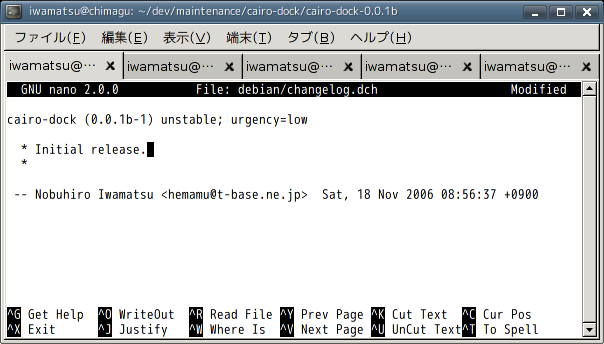
\includegraphics[width=0.5\hsize]{image200611/dch_image.png}
	\end{center}

	\item Upstream のソース変更

		そのままのソースコードでは パッケージ化した場合に不都合がある場合が多々あります。
		パッケージを作成する前に、Debian のパッケージ作成に合うように修正する必要があります。

		今回修正した点は以下のとおりです。

		\begin{itemize}
			\item Makefile の install ターゲットがないので追加します。
			\item Debian で配布されている libcarioパッケージの cairo-glitzが有効になってないので、
				Makefile の -DHAVE\_GLITZ を無効にします。

		変更前\\
		\begin{commandline}
APP = cairo-dock

CFLAGS  = `pkg-config --cflags cairo gtk+-2.0 librsvg-2.0 glitz-glx` -DHAVE_GLITZ
LDFLAGS = `pkg-config --libs   cairo gtk+-2.0 librsvg-2.0 glitz-glx` -lm

SRC = cairo-dock.c

all: $(APP)

clean:
        rm -f *.o *~ $(APP)
		\end{commandline}

		変更後\\
		\begin{commandline}
APP?=cairo-dock
BINDIR?=/usr/bin

CFLAGS  = `pkg-config --cflags cairo gtk+-2.0 librsvg-2.0 glitz-glx`
LDFLAGS = `pkg-config --libs   cairo gtk+-2.0 librsvg-2.0 glitz-glx` -lm

SRC = cairo-dock.c

all: $(APP)

clean:
        rm -f *.o *~ $(APP)

install:
        install -d ${DESTDIR}${BINDIR}
        install -m 755 cairo-dock ${DESTDIR}${BINDIR}

		\end{commandline}

			\item cairo-dock.c の画像ファイルの指定がプログラムのあるディレクトリになっているので修正します。


		\end{itemize} 


		直接ソース等を修正してもいいのですが、差分で管理するために diff を取り、dpatch で管理します。
		詳細は Debian 勉強会 2005年07月の資料\footnote{debianmeetingresume200507.pdf}にあります。

	\subsubsection{manpage の作成}		

		実行権限があるファイルに manpage がない場合作成し、パッケージで提供する必要があります。
				
	\item パッケージの作成

		debuild コマンドを使い、パッケージを作成します。

		\begin{commandline}
% debuild
 fakeroot debian/rules clean
dh_testdir
dh_testroot
rm -f build-stamp configure-stamp
# Add here commands to clean up after the build process.
/usr/bin/make clean
make[1]: ディレクトリ `/tmp/cairo-dock-0.0.1b' に入ります
rm -f *.o *~ cairo-dock
make[1]: ディレクトリ `/tmp/cairo-dock-0.0.1b' から出ます
dh_clean
 dpkg-source -b cairo-dock-0.0.1b
dpkg-source: building cairo-dock using existing cairo-dock_0.0.1b.orig.tar.gz
dpkg-source: building cairo-dock in cairo-dock_0.0.1b-1.diff.gz
dpkg-source: building cairo-dock in cairo-dock_0.0.1b-1.dsc
 debian/rules build
dh_testdir
# Add here commands to configure the package.
touch configure-stamp
dh_testdir
# Add here commands to compile the package.
/usr/bin/make
make[1]: ディレクトリ `/tmp/cairo-dock-0.0.1b' に入ります
cc `pkg-config --cflags cairo gtk+-2.0 librsvg-2.0 glitz-glx`   
	`pkg-config --libs   cairo gtk+-2.0 librsvg-2.0 glitz-glx` -lm  cairo-dock.c   -o cairo-dock
make[1]: ディレクトリ `/tmp/cairo-dock-0.0.1b' から出ます
#docbook-to-man debian/cairo-dock.sgml > cairo-dock.1
touch build-stamp
 fakeroot debian/rules binary
dh_testdir
dh_testroot
dh_clean -k
dh_installdirs
# Add here commands to install the package into debian/cairo-dock.
/usr/bin/make DESTDIR=/tmp/cairo-dock-0.0.1b/debian/cairo-dock install
make[1]: ディレクトリ `/tmp/cairo-dock-0.0.1b' に入ります
install -d /tmp/cairo-dock-0.0.1b/debian/cairo-dock/usr/bin
install -m 755 cairo-dock /tmp/cairo-dock-0.0.1b/debian/cairo-dock/usr/bin
install -d /tmp/cairo-dock-0.0.1b/debian/cairo-dock/usr/share/cairo-dock
install -m 666 *.svg /tmp/cairo-dock-0.0.1b/debian/cairo-dock/usr/share/cairo-dock
make[1]: ディレクトリ `/tmp/cairo-dock-0.0.1b' から出ます
dh_testdir
dh_testroot
dh_installchangelogs
dh_installdocs
dh_installexamples
dh_installman
dh_link
dh_strip
dh_compress
dh_fixperms
dh_installdeb
dh_shlibdeps
dh_gencontrol
dpkg-gencontrol: warning: unknown substitution variable ${misc:Depends}
dh_md5sums
dh_builddeb
dpkg-deb: `../cairo-dock_0.0.1b-1_i386.deb' にパッケージ `cairo-dock' を構築しています。
 dpkg-genchanges
dpkg-genchanges: including full source code in upload
dpkg-buildpackage (debuild emulation): full upload (original source is included)
Now running lintian...
W: cairo-dock: description-synopsis-might-not-be-phrased-properly
W: cairo-dock: wrong-bug-number-in-closes l3:#nnnn
Finished running lintian.
Now signing changes and any dsc files...
 signfile cairo-dock_0.0.1b-1.dsc Nobuhiro Iwamatsu <hemamu@t-base.ne.jp>

次のユーザーの秘密鍵のロックを解除するには
パスフレーズがいります:“Nobuhiro Iwamatsu <hemamu@t-base.ne.jp>”
1024ビットDSA鍵, ID 3170EBE9作成日付は2003-09-29


 signfile cairo-dock_0.0.1b-1_i386.changes Nobuhiro Iwamatsu <hemamu@t-base.ne.jp>

次のユーザーの秘密鍵のロックを解除するには
パスフレーズがいります:“Nobuhiro Iwamatsu <hemamu@t-base.ne.jp>”
1024ビットDSA鍵, ID 3170EBE9作成日付は2003-09-29


Successfully signed dsc and changes files

		\end{commandline}

	\end{enumerate}

\subsection{パッケージのテスト}
	パッケージができたから終わりなのではなく、できたパッケージの動作確認やパッケージ段階で不具合がないか、確認する必要があります。
	
	\subsubsection{pbuilder でビルドチェック}

		pbuilder\footnote{http://packages.qa.debian.org/p/pbuilder.html} は chrootシステムを構築し、その中でパッケージのビルドを行うツールです。
		最低限のユーザーランドの上で、パッケージの依存関係を解決し、パッケージをビルドできるの確認することができます。
		パッケージの依存関係に不備があった場合はパッケージがビルドできません。パッケージはできたが、実は自分の環境でしか
		ビルドできなかったという単純な問題を無くすために使用したほうがいいでしょう。

	\subsubsection{実際にインストールして、動作確認を行う}

		動作確認していないものを不特定多数の人に配布するのは問題ですので(やってない人もおられるようですが。)実際にインストール
		して、動作確認を行います。

		\begin{commandline}
# dpkg -i cairo-dock_0.0.1b-1_i386.deb
% cairo-dock 
		\end{commandline}

	\subsubsection{アンインストールできるか確認する}

		インストールした際にアンインストールスクリプトに不具合があり、正常にアンインストールできない
		場合があります。アンインストールもできるか確認します。

\subsection{まとめ}
	Debian パッケージを作成することは難しくなく、容易に作成できる環境は整っています。
	
	肝心なのはツールを使えるようになることではなく、Debian Policy をどれだけ熟読しているか、
	にかかってくるように思います。
	
	作って分からないことがあれば debian-devel@jp\footnote{debian-devel@debian.or.jp}等で聞くといいでしょう。	
	

\dancersection{sid を日常環境として使うための注意}{上川}
\label{sec:YYY}

\subsection{sid とはなにものか}

Debian sid は別名 unstable で、毎日リリースされている Debian の開発版で
す。開発者が新しいパッケージをリリースしたらまずそこに入ります。毎日日本
時間午前4時くらいに処理されており、そのタイミングで新しいバージョンが配
布されます。

開発者に近い層のユーザは、最新版のパッケージを利用するために unstable を
利用します。問題があれば随時バグ報告をしていきます。また、apt-listbugs
などを利用し、他のユーザから報告された深刻なバグがないか確認しながら作業
します。


\subsection{インストール方法}

毎日最新版になるので、安定して直接インストールできる方法というのは基本的
には無いでしょう。安定版をインストールしてから、 sid にアップグレードす
るという形が通常のやりかたです。

また、別の方法として、chroot 内部に sid を飼うという方法があります。
debootstrap や、 cdebootstrap などのツールを利用すると、 chroot 内部で
Debian sid が稼働している状況をつくれます。pbuilder などのツールを利用す
るとより便利に利用できます。

sid は最新版を常においかけているので、深刻なバグのリスクに出会う危険性が
常にあります。 chroot 内部で常に最新版を確認して、それを外部に展開すると
いうやりかたをしないと危険でしょう。

\subsection{魅力}

常に最新版が利用できます。開発が起きている場です。開発をしたいだとか、オー
プンソースの世界の動きを肌で感じたいというのであれば、お薦めです。

\subsection{情報源}

IRC や ML や 勉強会で情報収集しましょう。
\verb!#debian-devel! IRCチャンネルのトピックが一番最新の情報が得られます。

apt-listbugs や apt-listchanges というツールも利用しましょう。
apt-listbugs は今インストールしようとしているパッケージのバージョンに該
当する深刻なバグレポートを表示してくれるツールです。apt-listchanges  は
前回インストールしたバージョンからの changelog の差分を表示してくれるツー
ルです。

\dancersection{bugreport 論}{上川}

\subsection{Debian BTS の特徴}

Debian BTS は、ウェブとメールフロントエンドをもつバグトラッキングシステ
ムです。他のバグトラッキングシステムと違う点として、操作が全てメールでし
かできないという点と、情報が全て完全に公開されるという点があります。
また、バグレポートをパッケージ単位で分類しているという点も特徴です。

\subsection{使われ方}

深刻なバグ(RC バグ)を登録すると、そのパッケージのバージョンはリリース
できない、という意味になります。各ユーザはapt-listbugs を経由してそのよ
うなバグを確認し、深刻なバグのあるパッケージのバージョンをインストールし
ないように回避できます。また、この情報はリリースマネージメントにつかわれ
ています。

\subsection{アーキテクチャ}

バックエンドデータベースはプレーンのテキストファイルです。ファイル構造は
下記のようになっています。

\begin{itemize}
 \item /org/bugs.debian.org/spool
       \begin{itemize}
	\item incoming/
	\item db-h/
	      \begin{itemize}
	       \item 00/
		     \begin{itemize}
		      \item ..
		      \item 314200.log
		      \item 314200.report
		      \item 314200.status
		      \item 314200.summary
		     \end{itemize}
	       \item ..
	       \item 99/
	      \end{itemize}
	\item archive/
	      \begin{itemize}
	       \item 00/
	       \item ..
	       \item 99/
	      \end{itemize}
	\item index.db -- index.db.realtimeへのシンボリックリンク
	\item index.archive -- index.archive.realtimeへのシンボリックリ
	      ンク
	\item nextnumber
       \end{itemize}
\end{itemize}

メールを受信したら、そのメールが incoming 以下にスプールされます。
そのメールを15分に一回 cron から起動されるスクリプトが処理します。


ウェブ経由でバグ報告を確認するためのcgi があります。その cgi 経由では 
BTS は内容の閲覧だけができ、変更はしません。

また、スクリプトなどから利用するために、SOAP のフロントエンドがあります。
ドキュメントは一行もありません。

現状 \url{http://bugs.donarmstrong.com/cgi-bin/soap.cgi} でステージング
されています。今後は \url{http://bugs.debian.org} に移行したいようです。
ネームスペースは\url{Debbugs/SOAP/Status}で、そこで\verb!get_status!とい
う関数が定義されています。\verb!get_status!は複数の数字パラメータをうけ、
そのあたえられた数字に対応するバグレポートの情報をかえします。
\verb!get_status!は、バグ報告の本文ではなく、メタデータを返します。


\subsection{文化}

たまに BSP などの祭があります。バグトラッキングシステムに登録されている
バグで最初に対応されないものについては、そのまま放置され時間だけが過ぎて
しまう傾向があります。それらに対して新たな気持ちで対応しようというもので
す。

\subsection{参考文献}

\begin{itemize}
 \item Debian勉強会 2005年10月資料 「debbugs internal」
 \item Debian勉強会 2005年10月資料 「apt-listbugs の生い立ちと実装」
 \item \url{/usr/share/doc/debian/bug-maint-mailcontrol.txt}など
\end{itemize}

\dancersection{次回}{}

未定です。
内容は本日決定予定です。

参加者募集はまた後程。

\newpage

\vspace*{15cm}
\hrule
\vspace{2mm}

\includegraphics[width=2cm]{image200502/openlogo-nd.eps}
\noindent \Large \bf Debian 勉強会資料\\ \\
\noindent \normalfont 2006年11月19日 \hspace{5mm}  初版第1刷発行\\
\noindent \normalfont 東京エリア Debian 勉強会 (編集・印刷・発行)\\
\hrule

\end{document}
